% !TEX program = pdflatex
% Infographic poster (A0 portrait, 3 columns) built with the tikzposter class.
% Charts use pgfplots, the flow diagram and icons are drawn with TikZ, so the
% project needs no external images. Change the paper size with the class
% options (a0paper, a1paper, a2paper) and the content in the blocks below.
\documentclass[25pt, a0paper, portrait, margin=0mm, innermargin=15mm,
               blockverticalspace=15mm, colspace=15mm, subcolspace=8mm]{tikzposter}

\usepackage[utf8]{inputenc}
\usepackage[T1]{fontenc}
\usepackage[default]{lato}
\usepackage{amsmath}
\usepackage{booktabs}
\usepackage{enumitem}
\usepackage{pgfplots}
\pgfplotsset{compat=1.18}
\usetikzlibrary{arrows.meta,positioning,shapes.geometric,calc,shadows}

%---------------------------------------------------------------------
% Theme and palette
%---------------------------------------------------------------------
\definecolor{ink}{HTML}{1F2933}
\definecolor{teal}{HTML}{0B7285}
\definecolor{tealdark}{HTML}{095C6B}
\definecolor{sand}{HTML}{F8F4E8}
\definecolor{orange}{HTML}{E8590C}
\definecolor{sky}{HTML}{D0EBFF}

\definecolorstyle{LatexApi}{
  \definecolor{colorOne}{named}{teal}
  \definecolor{colorTwo}{named}{sand}
  \definecolor{colorThree}{named}{orange}
}{
  \colorlet{backgroundcolor}{sand}
  \colorlet{framecolor}{teal}
  \colorlet{titlefgcolor}{white}
  \colorlet{titlebgcolor}{teal}
  \colorlet{blocktitlebgcolor}{teal}
  \colorlet{blocktitlefgcolor}{white}
  \colorlet{blockbodybgcolor}{white}
  \colorlet{blockbodyfgcolor}{ink}
  \colorlet{innerblocktitlebgcolor}{sky}
  \colorlet{innerblocktitlefgcolor}{ink}
  \colorlet{innerblockbodybgcolor}{sky!50}
  \colorlet{innerblockbodyfgcolor}{ink}
  \colorlet{notefgcolor}{ink}
  \colorlet{notebgcolor}{orange!20}
  \colorlet{noteframecolor}{orange}
}
\usetheme{Simple}
\usecolorstyle{LatexApi}
\useblockstyle{Default}
\usetitlestyle{Filled}

% remove the "LaTeX TikZposter" stamp in the corner
\tikzposterlatexaffectionproofoff

%---------------------------------------------------------------------
% Reusable TikZ icons (no icon fonts needed in pdflatex)
%---------------------------------------------------------------------
\newcommand{\icondoc}[1][teal]{%
  \begin{tikzpicture}[scale=0.9]
    \draw[#1, line width=3pt, fill=white] (0,0) -- (0,3) -- (1.6,3) -- (2.4,2.2) -- (2.4,0) -- cycle;
    \draw[#1, line width=3pt] (1.6,3) -- (1.6,2.2) -- (2.4,2.2);
    \foreach \y in {0.6,1.1,1.6} \draw[#1, line width=2.5pt] (0.4,\y) -- (2,\y);
  \end{tikzpicture}}
\newcommand{\icongearbig}[1][teal]{%
  \begin{tikzpicture}[scale=0.9]
    \fill[#1] (1.2,1.5) circle (1.0);
    \foreach \a in {0,45,...,315} \fill[#1, rotate around={\a:(1.2,1.5)}] (1.05,2.3) rectangle (1.35,2.8);
    \fill[white] (1.2,1.5) circle (0.4);
  \end{tikzpicture}}
\newcommand{\iconpdf}[1][orange]{%
  \begin{tikzpicture}[scale=0.9]
    \draw[#1, line width=3pt, fill=white] (0,0) -- (0,3) -- (1.6,3) -- (2.4,2.2) -- (2.4,0) -- cycle;
    \node[#1, font=\bfseries\large] at (1.2,1.1) {PDF};
  \end{tikzpicture}}
\newcommand{\iconfont}[1][teal]{%
  \begin{tikzpicture}[scale=0.9]
    \draw[#1, line width=3pt, rounded corners=4pt] (0,0) rectangle (2.4,3);
    \node[#1, font=\bfseries\Huge] at (1.2,1.5) {Aa};
  \end{tikzpicture}}
\newcommand{\iconterminal}[1][teal]{%
  \begin{tikzpicture}[scale=0.9]
    \draw[#1, line width=3pt, rounded corners=4pt, fill=white] (0,0) rectangle (3,2.4);
    \fill[#1] (0,1.9) rectangle (3,2.4);
    \draw[#1, line width=3pt] (0.4,1.4) -- (0.9,1.0) -- (0.4,0.6);
    \draw[#1, line width=3pt] (1.1,0.6) -- (1.9,0.6);
  \end{tikzpicture}}

%---------------------------------------------------------------------
% Title
%---------------------------------------------------------------------
\title{\parbox{0.9\linewidth}{\centering How a \LaTeX{} Document Becomes a PDF}}
\author{Alex Rivera \quad Jordan Lee \quad Sam Okafor}
\institute{Example University \,\textbullet\, Example Labs \,\textbullet\, Open Lab Workshop Series}
\titlegraphic{\icondoc[white]}

\begin{document}
\maketitle[width=0.95\linewidth, titletotopverticalspace=20mm, titletoblockverticalspace=25mm]

\begin{columns}

%=====================================================================
\column{0.33}
%=====================================================================

\block{1. From source to typeset boxes}{
  A \LaTeX{} file is plain text. The engine reads it character by character,
  turns it into \emph{tokens}, expands macros and finally produces
  \emph{boxes}: rectangles with a width, a height and a depth. Paragraphs are
  broken into lines by an optimal line-breaking algorithm, and pages are built
  by stacking boxes until the page is full.

  \vspace{1em}
  \begin{tikzfigure}[Tokens become boxes, boxes become pages.]
    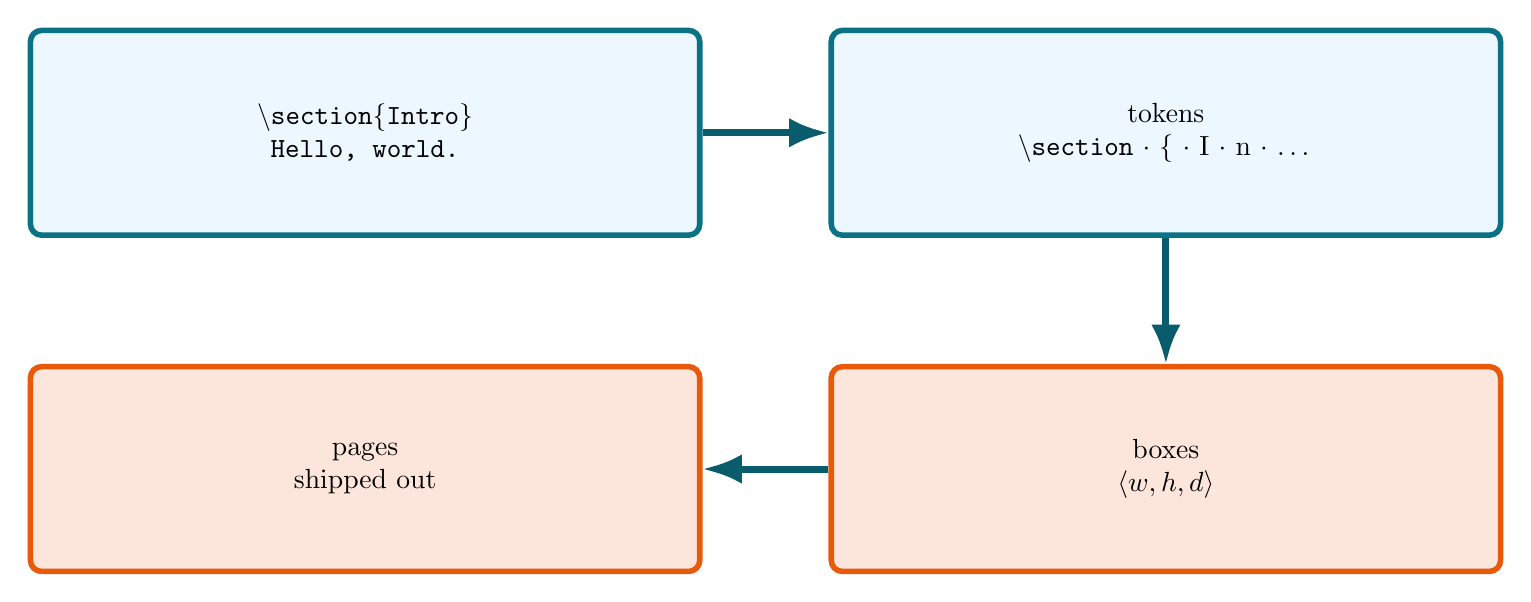
\begin{tikzpicture}[font=\normalsize, node distance=16mm]
      \node[draw=teal, line width=2pt, rounded corners, fill=sky!40, minimum width=85mm, minimum height=26mm, align=center] (src) {\texttt{\textbackslash section\{Intro\}}\\\texttt{Hello, world.}};
      \node[draw=teal, line width=2pt, rounded corners, fill=sky!40, minimum width=85mm, minimum height=26mm, align=center, right=of src] (tok) {tokens\\\texttt{\textbackslash section} $\cdot$ \texttt{\{} $\cdot$ I $\cdot$ n $\cdot$ \ldots};
      \node[draw=orange, line width=2pt, rounded corners, fill=orange!15, minimum width=85mm, minimum height=26mm, align=center, below=of tok] (box) {boxes\\$\langle w, h, d\rangle$};
      \node[draw=orange, line width=2pt, rounded corners, fill=orange!15, minimum width=85mm, minimum height=26mm, align=center, left=of box] (page) {pages\\shipped out};
      \draw[-{Latex[length=5mm]}, line width=2.5pt, tealdark] (src) -- (tok);
      \draw[-{Latex[length=5mm]}, line width=2.5pt, tealdark] (tok) -- (box);
      \draw[-{Latex[length=5mm]}, line width=2.5pt, tealdark] (box) -- (page);
    \end{tikzpicture}
  \end{tikzfigure}
}

\block{2. Three engines, one language}{
  \begin{center}
  \small
  \setlength{\tabcolsep}{10pt}
  \begin{tabular}{@{}lccc@{}}
    \toprule
    & \textbf{pdfTeX} & \textbf{XeTeX} & \textbf{LuaTeX} \\
    \midrule
    Output & PDF & XDV $\to$ PDF & PDF \\
    Input encoding & \texttt{inputenc} & UTF-8 & UTF-8 \\
    Fonts & Type\,1 & OpenType & OpenType \\
    Scripting & -- & -- & Lua \\
    Start-up & fastest & fast & slowest \\
    \bottomrule
  \end{tabular}
  \end{center}

  \vspace{1em}
  \begin{tikzfigure}[Median compile time of an 8-page paper (seconds).]
    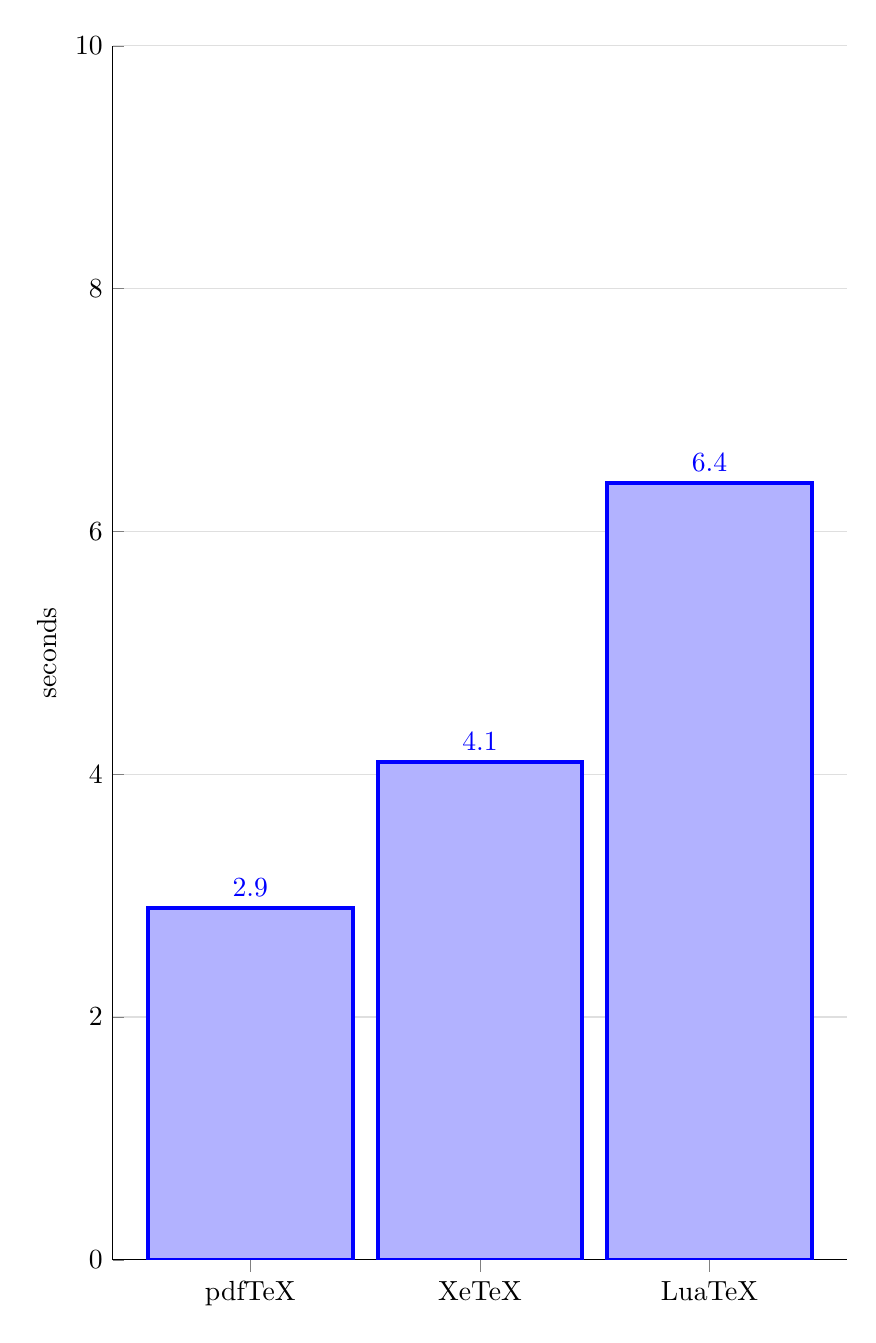
\begin{tikzpicture}
      \begin{axis}[
          ybar, bar width=26mm, width=0.9\linewidth, height=170mm,
          ymin=0, ymax=10, ytick={0,2,4,6,8,10}, ylabel={seconds},
          symbolic x coords={pdfTeX, XeTeX, LuaTeX}, xtick=data,
          nodes near coords, nodes near coords style={font=\normalsize},
          axis lines*=left, ymajorgrids, grid style={gray!25},
          every axis plot/.append style={fill=teal, draw=tealdark, line width=1.5pt},
          enlarge x limits=0.3,
        ]
        \addplot coordinates {(pdfTeX,2.9) (XeTeX,4.1) (LuaTeX,6.4)};
      \end{axis}
    \end{tikzpicture}
  \end{tikzfigure}
}

\block{3. Fonts}{
  \begin{minipage}{0.22\linewidth}\centering\iconfont\end{minipage}%
  \begin{minipage}{0.76\linewidth}
    pdfTeX embeds \textbf{Type\,1} fonts described by metric files
    (\texttt{.tfm}); XeTeX and LuaTeX load \textbf{OpenType} fonts directly
    through \texttt{fontspec}. Every glyph used in the document is embedded in
    the PDF, which is why a 2-page paper can weigh 150~kB.
  \end{minipage}
}

\block{Glossary}{
  \begin{description}[style=unboxed, font=\bfseries\color{teal}, leftmargin=0pt, labelsep=0.8em, itemsep=4pt]
    \item[Format file] A pre-digested dump of the \LaTeX{} kernel that the
      engine loads at start-up instead of re-reading thousands of macros.
    \item[\texttt{.aux}] Auxiliary file where labels, citations and counters
      are written for the next pass.
    \item[\texttt{.bbl}] Formatted bibliography produced by \texttt{bibtex}
      or \texttt{biber} from your \texttt{.bib} entries.
    \item[Glyph] The drawn shape of a character inside a font; only the
      glyphs you use are embedded.
  \end{description}
}

%=====================================================================
\column{0.34}
%=====================================================================

\block{4. The build pipeline}{
  Most documents need \textbf{more than one pass}: the first run writes
  labels, citations and the table of contents to auxiliary files, and later
  runs read them back. \texttt{latexmk} automates the loop and decides when
  to call \texttt{bibtex} or \texttt{biber}.

  \vspace{1em}
  \begin{tikzfigure}[A typical multi-pass build driven by latexmk.]
    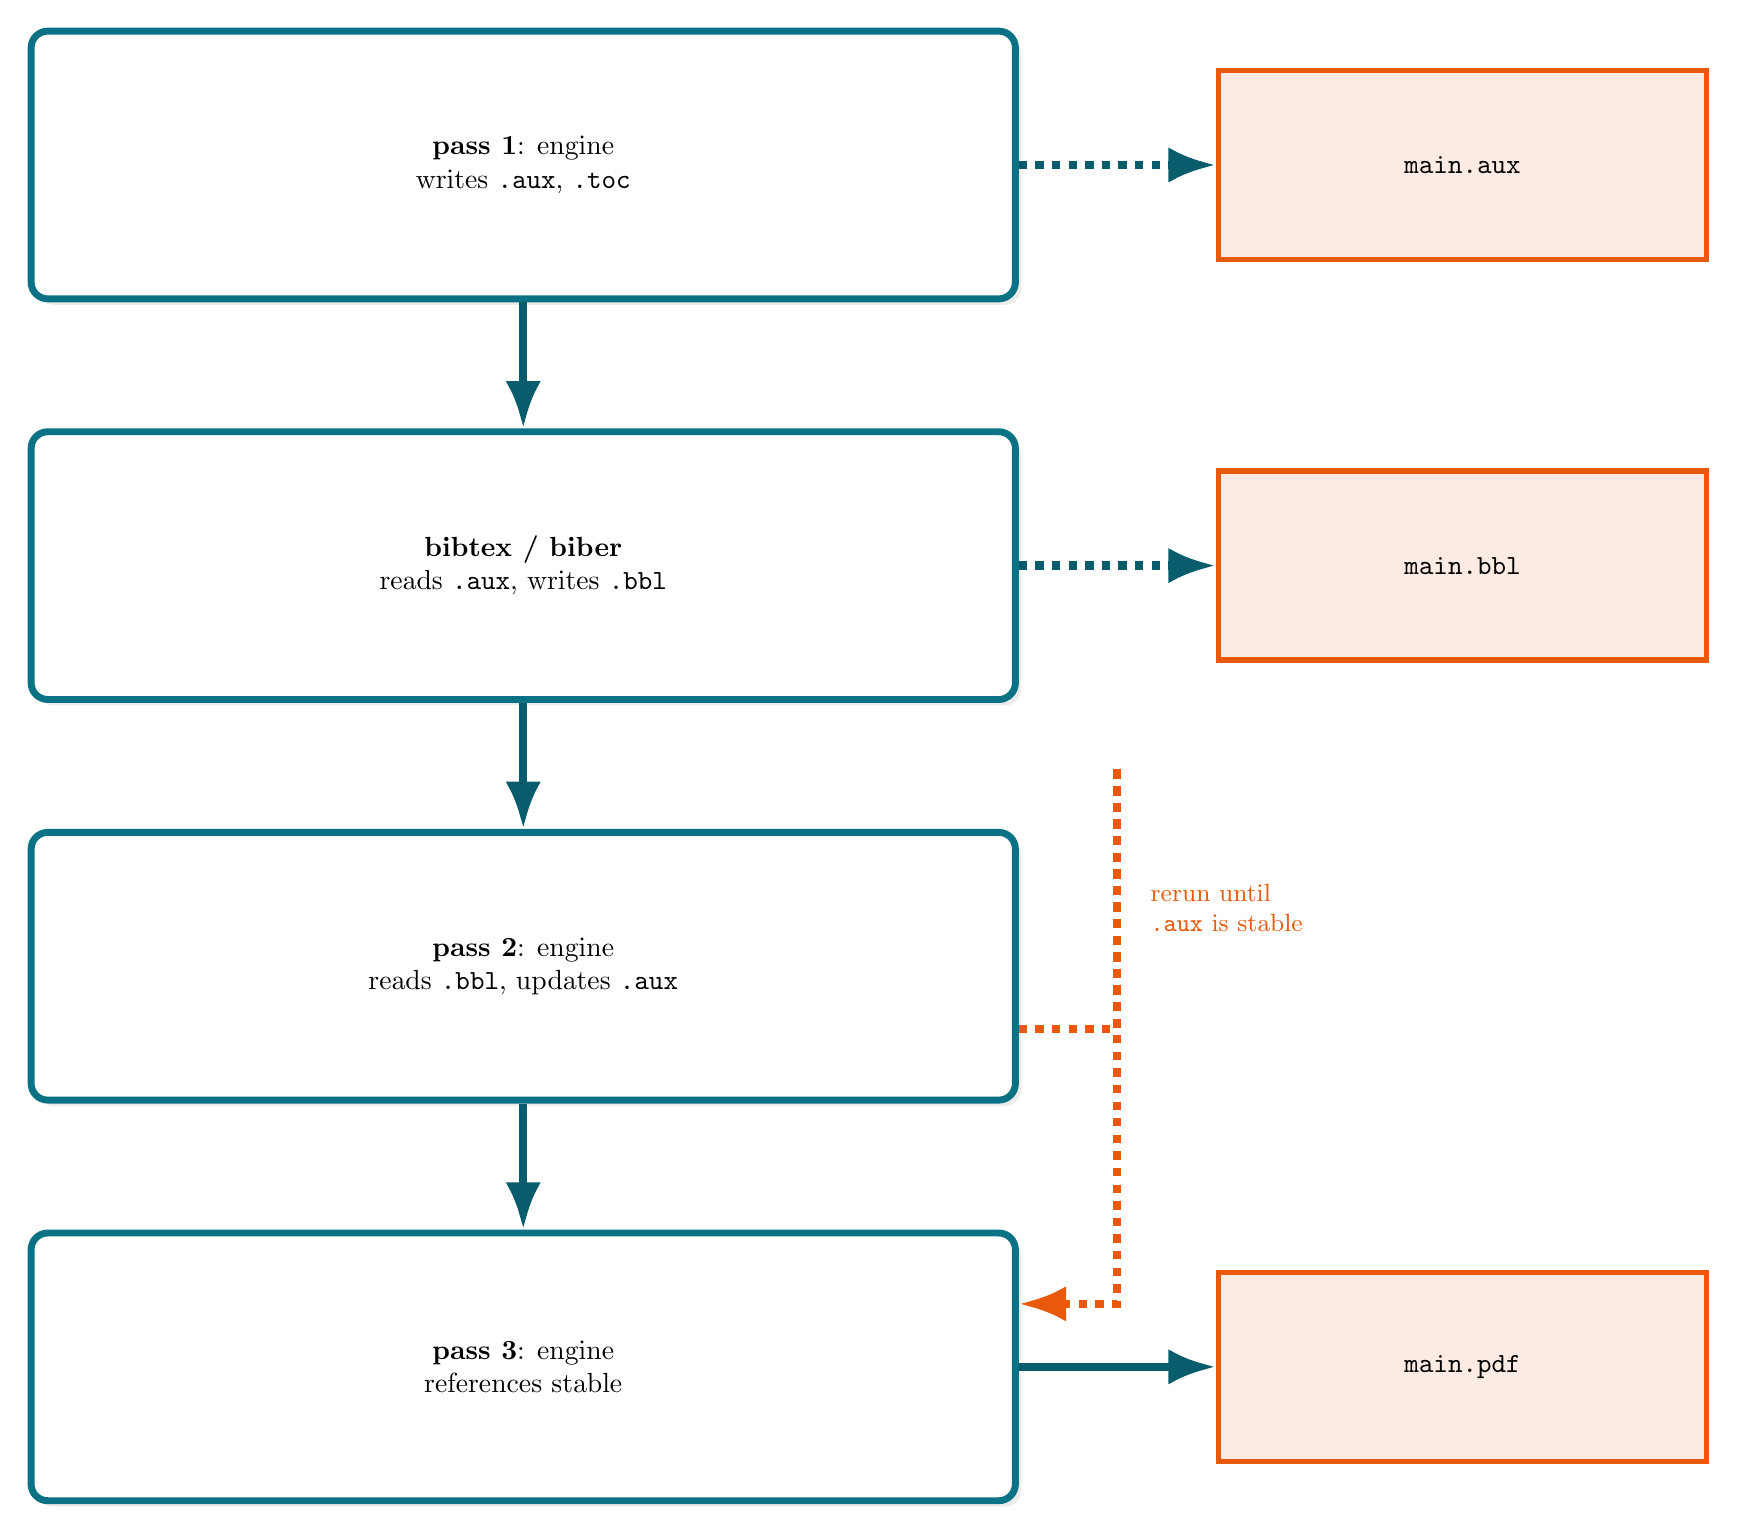
\begin{tikzpicture}[
        font=\normalsize, node distance=16mm,
        stage/.style={draw=teal, line width=2.5pt, rounded corners=6pt, fill=white,
                      minimum width=125mm, minimum height=34mm, align=center, drop shadow={opacity=0.15}},
        file/.style={draw=orange, line width=2pt, fill=orange!12, align=center,
                     minimum width=62mm, minimum height=24mm},
        arr/.style={-{Latex[length=6mm]}, line width=3pt, tealdark},
      ]
      \node[stage] (p1) {\textbf{pass 1}: engine\\writes \texttt{.aux}, \texttt{.toc}};
      \node[stage, below=of p1] (bib) {\textbf{bibtex / biber}\\reads \texttt{.aux}, writes \texttt{.bbl}};
      \node[stage, below=of bib] (p2) {\textbf{pass 2}: engine\\reads \texttt{.bbl}, updates \texttt{.aux}};
      \node[stage, below=of p2] (p3) {\textbf{pass 3}: engine\\references stable};
      \node[file, right=25mm of p1] (aux) {\texttt{main.aux}};
      \node[file, right=25mm of bib] (bbl) {\texttt{main.bbl}};
      \node[file, right=25mm of p3] (pdf) {\texttt{main.pdf}};
      \draw[arr] (p1) -- (bib);
      \draw[arr] (bib) -- (p2);
      \draw[arr] (p2) -- (p3);
      \draw[arr, dashed] (p1) -- (aux);
      \draw[arr, dashed] (bib) -- (bbl);
      \draw[arr] (p3) -- (pdf);
      \draw[arr, dashed, orange] (p2.east) ++(0,-8mm) -| ($(p2.east)!0.5!(bbl.west)$) |- ($(p3.east)+(0,8mm)$);
      \node[orange, font=\small, align=left, anchor=west] at ($(p2.east)!0.5!(bbl.west) + (3mm,-18mm)$) {rerun until\\\texttt{.aux} is stable};
    \end{tikzpicture}
  \end{tikzfigure}
}

\block{5. Where the time goes}{
  \begin{tikzfigure}[Cumulative time of a cold build inside a container.]
    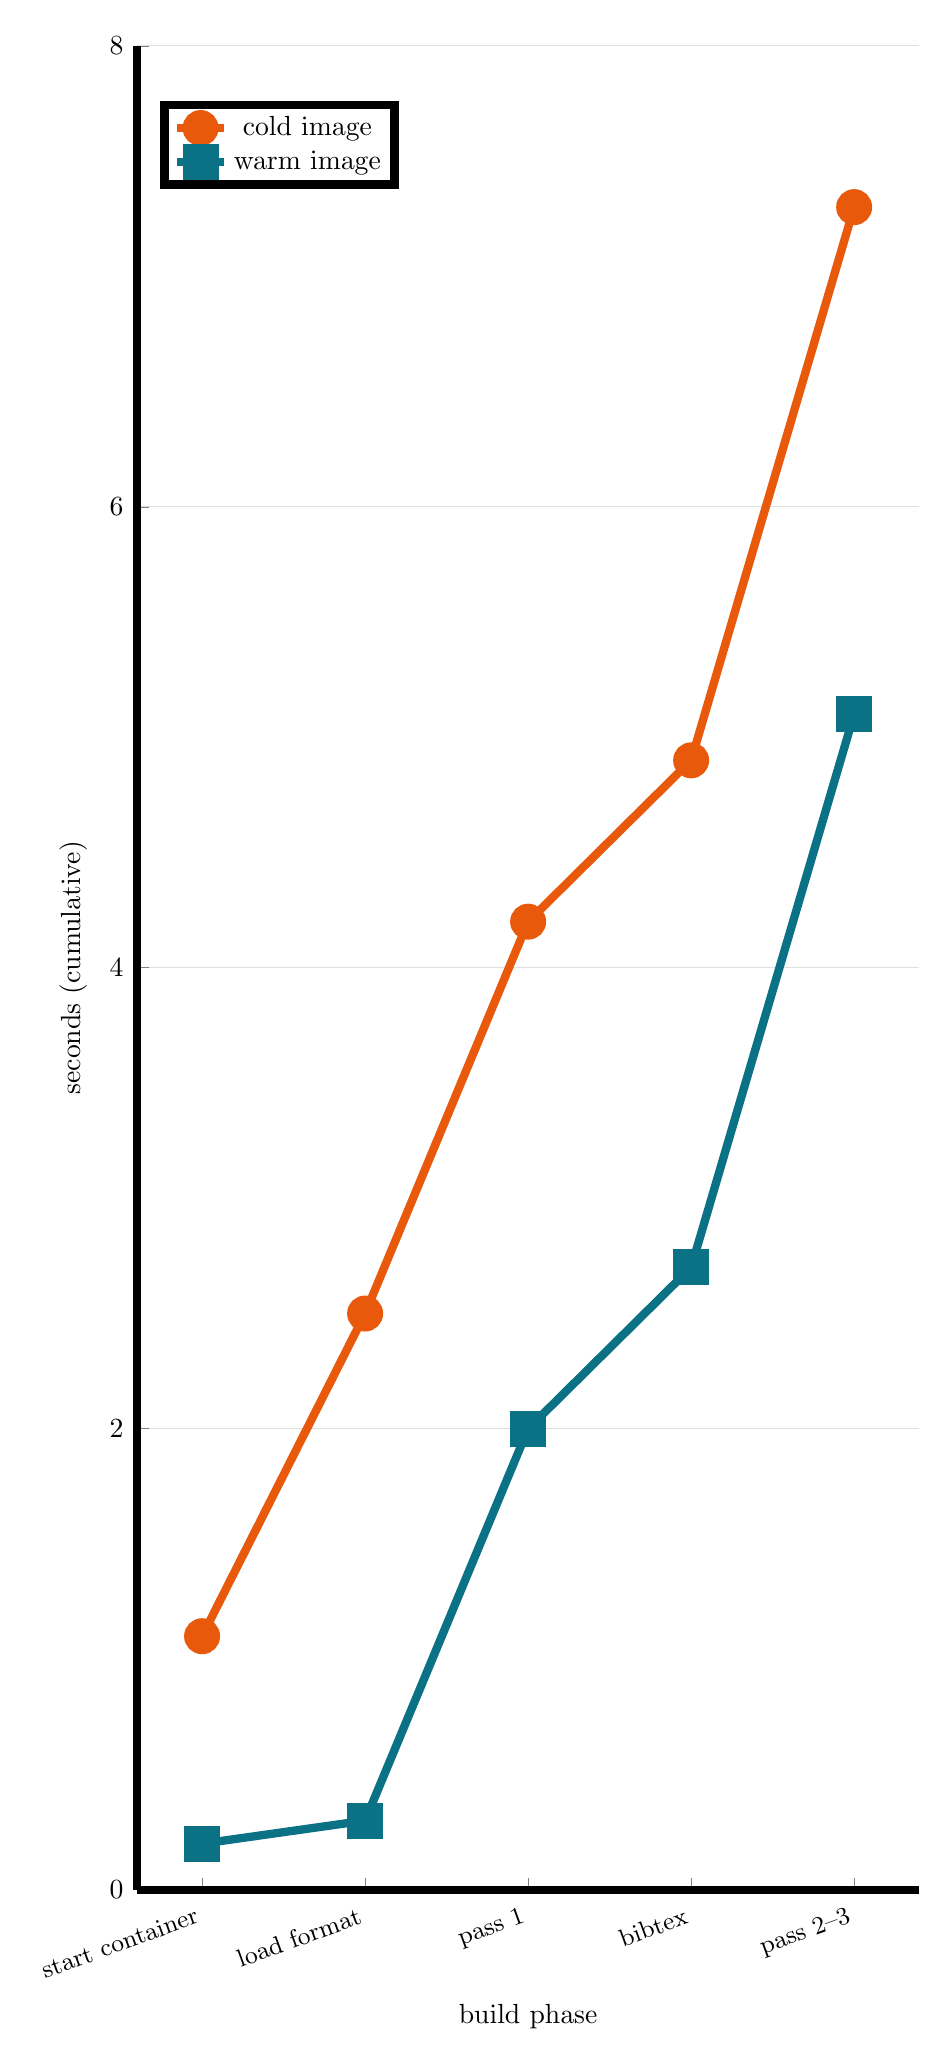
\begin{tikzpicture}
      \begin{axis}[
          width=0.95\linewidth, height=250mm,
          xlabel={build phase}, ylabel={seconds (cumulative)},
          xtick={1,...,5},
          xticklabels={start container, load format, pass 1, bibtex, pass 2--3},
          x tick label style={rotate=20, anchor=north east, font=\small},
          ymin=0, ymax=8, ytick={0,2,4,6,8}, ymajorgrids, grid style={gray!25},
          axis lines*=left, legend pos=north west, legend style={font=\normalsize},
          line width=3pt, mark size=5pt,
        ]
        \addplot[color=orange, mark=*] coordinates {(1,1.1) (2,2.5) (3,4.2) (4,4.9) (5,7.3)};
        \addplot[color=teal, mark=square*] coordinates {(1,0.2) (2,0.3) (3,2.0) (4,2.7) (5,5.1)};
        \legend{cold image, warm image}
      \end{axis}
    \end{tikzpicture}
  \end{tikzfigure}

  \vspace{0.5em}
  Pre-generating the format files and the font database inside the image
  removes most of the fixed start-up cost. The engine passes themselves
  take about the same time either way.
}

\block{Try it yourself}{
  \begin{minipage}{0.22\linewidth}\centering\iconterminal\end{minipage}%
  \begin{minipage}{0.76\linewidth}
    One command is enough on any machine with \TeX{} Live installed. It runs
    the engine as many times as needed and calls the bibliography tool for
    you:
  \end{minipage}

  \vspace{0.8em}
  \begin{center}
    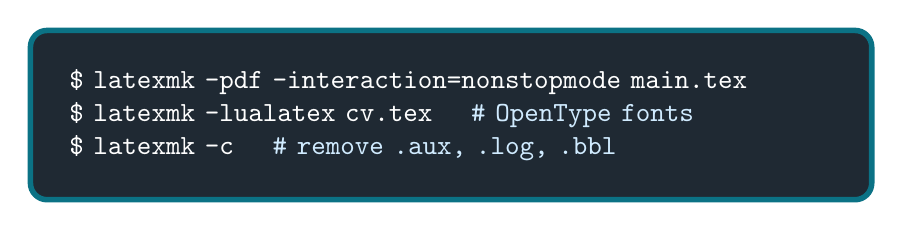
\begin{tikzpicture}
      \node[draw=teal, line width=2pt, rounded corners=6pt, fill=ink, text=white,
            font=\ttfamily\normalsize, inner sep=14pt, align=left, text width=0.8\linewidth] {%
        \$ latexmk -pdf -interaction=nonstopmode main.tex\\
        \$ latexmk -lualatex cv.tex \quad\textcolor{sky}{\# OpenType fonts}\\
        \$ latexmk -c \quad\textcolor{sky}{\# remove .aux, .log, .bbl}};
    \end{tikzpicture}
  \end{center}
}

%=====================================================================
\column{0.33}
%=====================================================================

\block{6. Inside the PDF}{
  \begin{minipage}{0.22\linewidth}\centering\iconpdf\end{minipage}%
  \begin{minipage}{0.76\linewidth}
    The final file is a tree of \textbf{objects}: a catalog, a page tree, one
    content stream per page, embedded font programs and, optionally, an
    outline, hyperlinks and metadata. pdfTeX compresses streams and can pack
    small objects into \emph{object streams}, which is why the page count is
    not visible in a plain-text search.
  \end{minipage}

  \vspace{1em}
  \begin{tikzfigure}[Object graph of a minimal two-page PDF.]
    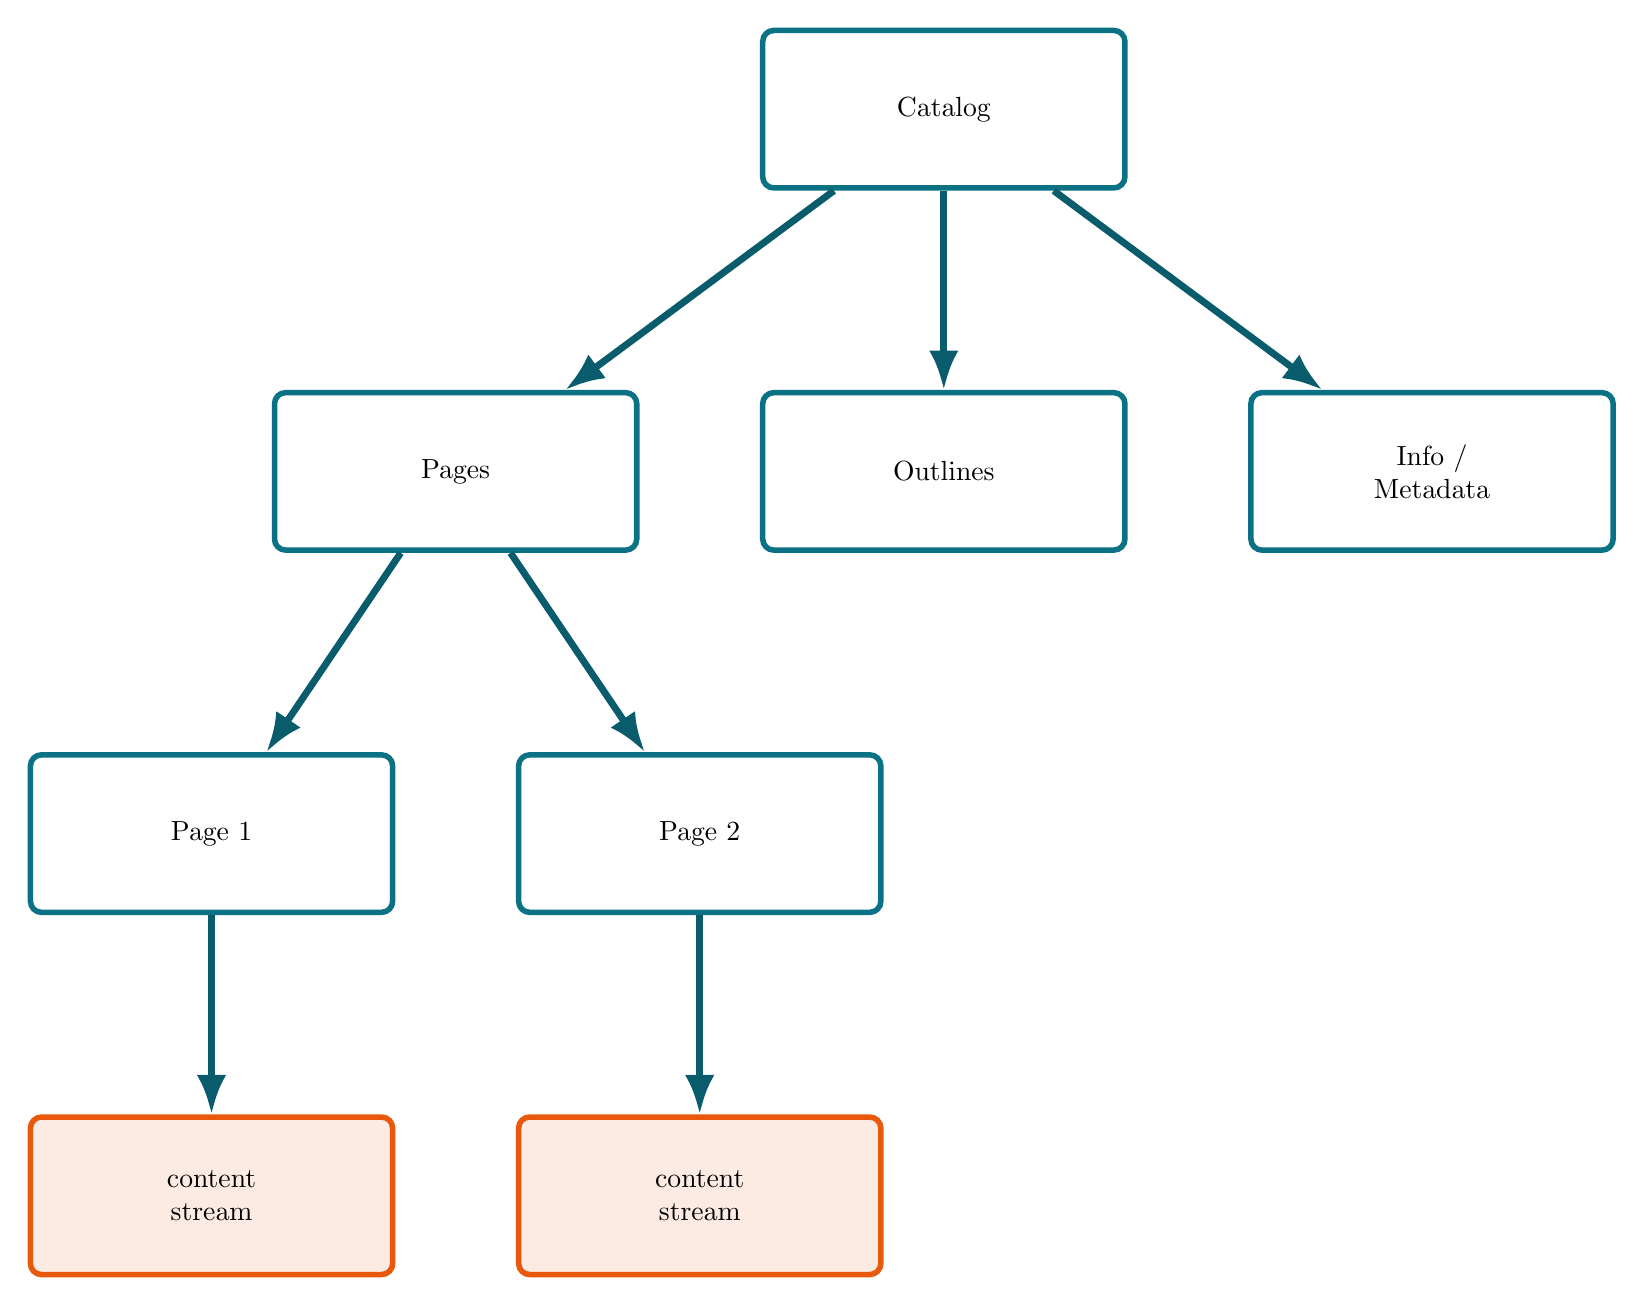
\begin{tikzpicture}[
        font=\normalsize, level distance=46mm, sibling distance=62mm,
        every node/.style={draw=teal, line width=2pt, rounded corners=4pt, fill=white, align=center, minimum width=46mm, minimum height=20mm},
        edge from parent/.style={draw=tealdark, line width=2.5pt, -{Latex[length=5mm]}},
      ]
      \node {Catalog}
        child { node {Pages}
          child { node {Page 1} child { node[fill=orange!12, draw=orange] {content\\stream} } }
          child { node {Page 2} child { node[fill=orange!12, draw=orange] {content\\stream} } }
        }
        child { node {Outlines} }
        child { node {Info /\\Metadata} };
    \end{tikzpicture}
  \end{tikzfigure}
}

\block{7. Running it in the cloud}{
  \begin{minipage}{0.22\linewidth}\centering\icongearbig\end{minipage}%
  \begin{minipage}{0.76\linewidth}
    A compile service treats the project as an \textbf{immutable bundle}: its
    hash identifies the output, so unchanged documents are never rebuilt.
    Each build runs in a throw-away container with no network, no shell
    escape and strict CPU, memory and time limits.
  \end{minipage}

  \vspace{1em}
  \innerblock{Safety checklist}{
    \begin{itemize}
      \item Unprivileged user, read-only root file system
      \item \texttt{-{}-network none}, seccomp allow-list
      \item \texttt{shell\_escape = f}, \texttt{openout\_any = p}
      \item 2~GB memory, 2 CPUs, 64 processes, hard timeout
    \end{itemize}
  }

  \vspace{1em}
  \begin{center}
    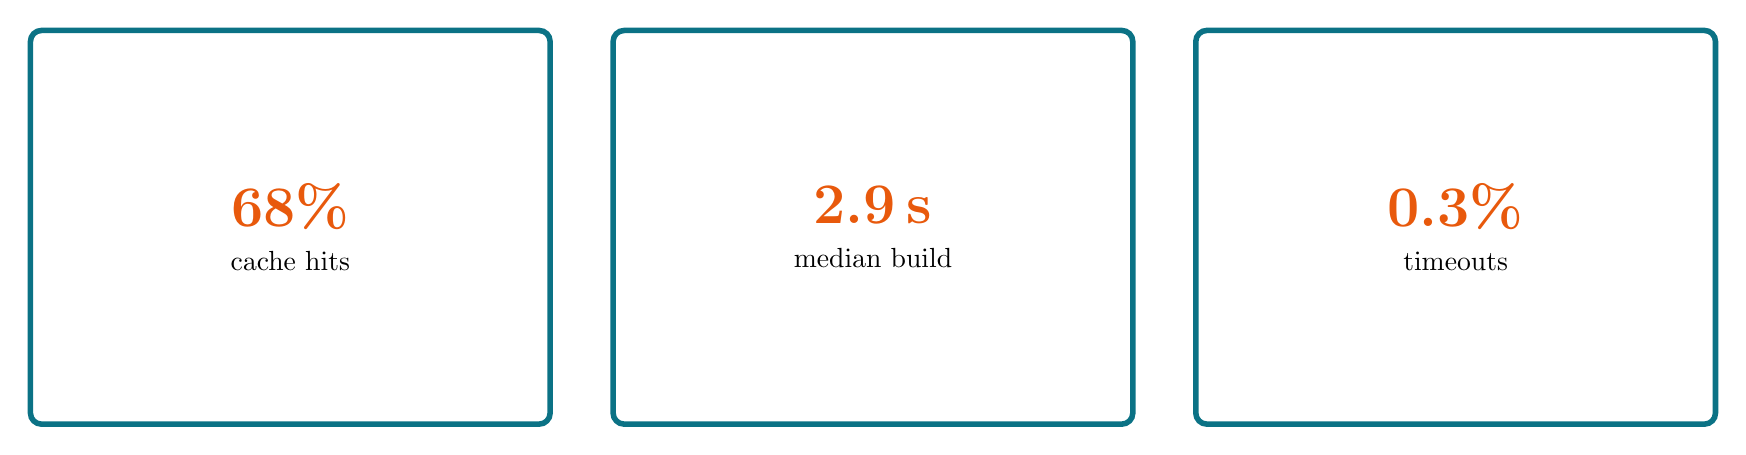
\begin{tikzpicture}[font=\normalsize]
      \foreach \v/\l/\i in {68\%/cache hits/0, 2.9\,s/median build/1, 0.3\%/timeouts/2} {
        \node[draw=teal, line width=2pt, rounded corners=4pt, minimum width=66mm, minimum height=50mm,
              align=center, fill=white] at (\i*74mm,0)
              {{\color{orange}\huge\bfseries\v}\\[4pt]\l};
      }
    \end{tikzpicture}
  \end{center}
}

\block{Take-aways}{
  \begin{enumerate}
    \item \LaTeX{} is a programming language whose output is boxes.
    \item Multi-pass builds are normal; let \texttt{latexmk} drive them.
    \item Fonts are embedded, so the PDF is self-contained.
    \item In the cloud, start-up cost dominates short builds; cache
      aggressively and warm the image.
  \end{enumerate}

  \vspace{0.5em}
  {\small\color{gray} Poster template for the latex-api project. Built with
  tikzposter and pgfplots; all figures are drawn with TikZ and the data is
  fictional, for illustration only.}
}

\end{columns}

\end{document}
